\documentclass[11pt]{article}
\usepackage[margin=1in]{geometry}
\usepackage{amsmath,amssymb,graphicx,hyperref,tikz}
\usetikzlibrary{positioning,arrows.meta}
\title{SIMBA: Methodology and Mathematical Scope}
\author{Ajit Kumar}
\date{Research implementation; October 2026}
\begin{document}
\maketitle
\begin{abstract}
SIMBA separates joint bundle incidence, redundancy-aware seed concordance and
exposure-modulated Gaussian shrinkage. This document specifies the implemented
method and its assumptions. It accompanies the software and is not a claim of
a peer-reviewed publication.
\end{abstract}
% ======================================================================
%  METHOD
% ======================================================================
\section{Method}
\label{sec:method}

To avoid conflating distinct notions of multi-item ``synergy,'' \textsc{SIMBA} isolates three distinct
mathematical estimators on top of a unified pairwise baseline, each addressing a specific failure mode of linear
bundle recommenders:
\begin{enumerate}\itemsep1pt
  \item \textbf{Simplicial Hyperedge Incidence Surplus} ($\hat{\Delta}_{\text{inc}}$, \S\ref{sec:incidence}):
  retains which items occurred together inside the \emph{same} historical bundle ($\lvert b \cap S\rvert \ge 2$),
  preserving $(k \ge 3)$-way joint incidence information that is destroyed by the pairwise projection $C = B^{\!\top} B$
  and vanishing identically on single-seed queries ($\lvert S\rvert = 1$).
  \item \textbf{Redundancy-Corrected Quadratic Concordance} ($\hat{R}_{\gamma}$, \S\ref{sec:concordance}):
  aggregates pairwise candidate--seed supports $w_{c,s}$ nonlinearly via \emph{Rao's quadratic diversity}
  (Rao, 1982) over a seed-redundancy kernel $G_S$, capturing second-order \emph{pairwise seed agreement} while
  discounting redundant query seeds.
  \item \textbf{Exposure-Modulated Conjugate Empirical-Bayes Shrinkage} ($\hat{\theta}_{S,c}$, \S\ref{sec:eb}):
  estimates an identifiable target---standardized latent compatibility $\theta_{S,c}$---via the exact conjugate
  normal--normal posterior $\hat{\theta}_{S,c} = (1 - u_c)Y(c\mid S) + u_c\mu_0(c\mid S)$ using a
  validation-frozen prior scale and constrained OLS variance-component estimation on $1/f_c$.
\end{enumerate}
Figure~\ref{fig:framework} summarises the architecture. All supporting components (taxonomic compatibility
including additive diagonal self-exclusion, style-disentangled content, bilateral graph-bridged representations,
and a lightweight $0.10\text{M}$--$0.30\text{M}$ set-attention contrastive encoder) enter the pairwise baseline
first, ensuring that ablations of $\hat{\Delta}_{\text{inc}}$, $\hat{R}_{\gamma}$, and $\hat{\theta}_{S,c}$ are
strictly unconfounded.

\begin{figure}[t]
  \centering
  \resizebox{\linewidth}{!}{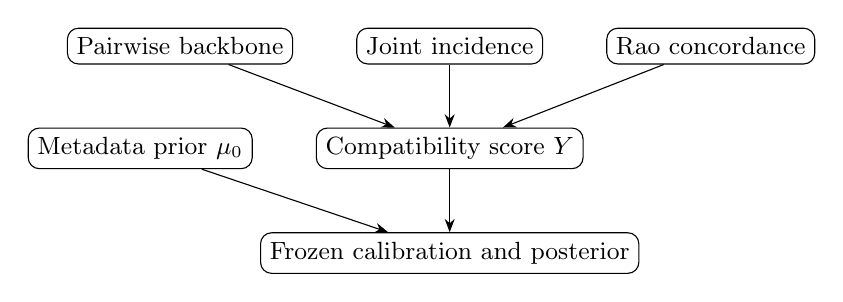
\begin{tikzpicture}[node distance=8mm, every node/.style={draw,rounded corners,align=center,font=\small}, >={Stealth}]
\node (base) {Pairwise backbone};
\node[right=of base] (inc) {Joint incidence};
\node[right=of inc] (rao) {Rao concordance};
\node[below=of inc] (score) {Compatibility score $Y$};
\node[left=of score] (prior) {Metadata prior $\mu_0$};
\node[below=of score] (post) {Frozen calibration and posterior};
\draw[->] (base)--(score);
\draw[->] (inc)--(score);
\draw[->] (rao)--(score);
\draw[->] (score)--(post);
\draw[->] (prior)--(post);
\end{tikzpicture}
}
  \caption{Overview of \textsc{SIMBA}. First-order pairwise channels are augmented by two orthogonal multi-seed
  estimators---Simplicial Hyperedge Incidence Surplus ($\hat{\Delta}_{\text{inc}}$) and Redundancy-Corrected
  Quadratic Concordance ($\hat{R}_{\gamma}$)---followed by Exact Exposure-Modulated Conjugate Empirical-Bayes
  Shrinkage ($\hat{\theta}_{S,c} = (1-u_c)Y + u_c\mu_0$).}
  \label{fig:framework}
\end{figure}

\subsection{Problem Formulation and Pairwise Baseline}
\label{sec:prob}
Let $\mathcal{I}$ ($|\mathcal{I}|=n$) be the item catalogue and $\mathcal{B}_{\text{train}}$ the training bundles
with incidence matrix $B\in\{0,1\}^{|\mathcal{B}_{\text{train}}|\times n}$, item frequencies
$f_i = \sum_{b} B_{b,i}$, and bundle sizes $|b| = \sum_i B_{b,i}$. Given a partial query bundle $S \subset b$,
the goal is to rank all candidates $c \in \mathcal{I}\setminus S$ to recover $b\setminus S$.

A standard pairwise recommender depends only on the 1-skeleton projection $C = B^{\!\top}B - \operatorname{diag}$
or degree-normalised pairwise transitions
$W_{\text{pair}} = B^{\!\top}\operatorname{diag}\big((|b|+1)^{-\gamma_{\text{vol}}}\big)B\operatorname{diag}\big((f+\alpha_0)^{-\alpha_{\text{deg}}}\big)$
($\operatorname{diag}(W_{\text{pair}})=0$), scoring candidates additively across seeds:
\begin{equation}
  s_{\text{pair}}(c\mid S) = \sum_{s\in S} (W_{\text{pair}})_{c,s}.
  \label{eq:pair}
\end{equation}
Two-hop collaborative smoothing is performed via the exact zero-diagonal \emph{row-stochastic} bipartite random
walk $P_{\text{rw}} = D_{\text{row}}^{-1}(D_I^{-1}B^{\!\top}D_B^{-1}B - \operatorname{diag})$ (where every active
item row sums to $1$) or its variance-stabilised symmetric counterpart. Alongside collaborative transitions, the
pairwise baseline includes dual-spectrum taxonomic PMI $P_{\text{cat}}$ (with additive diagonal self-exclusion for
low-duplication categories), style-disentangled content $\tilde{x}_i = x_i - \bar{x}_{\text{cat}(i)}$,
graph-bridged content, and a lightweight set-attention contrastive encoder (\S\ref{sec:reasoner}).

\subsection{Estimator I: Simplicial Hyperedge Incidence Surplus}
\label{sec:incidence}
The pairwise operator~\eqref{eq:pair} cannot distinguish whether a candidate $c$ co-occurred with two seeds
$s_1, s_2 \in S$ \emph{simultaneously in the same historical bundle} $b \supset \{c, s_1, s_2\}$ or merely in two
separate bundles $b_1 \supset \{c, s_1\}$ and $b_2 \supset \{c, s_2\}$. To isolate true $(k \ge 3)$-way joint
co-occurrence in $B$ from the pairwise base~\eqref{eq:pair}, we define the pure \emph{simplicial incidence
surplus} (\texttt{score\_simplicial\_incidence\_only}):
\begin{equation}
  \hat{\Delta}_{\text{inc}}(c\mid S)
  = \sum_{b \in \mathcal{B}_{\text{train}} : c \in b}
    (|b|+1)^{-\gamma_{\text{vol}}}
    \Big(\sum_{s\in b\cap S}(f_s+\alpha_0)^{-\alpha_{\text{deg}}}\Big)\,
    \beta_{\text{clique}}\max\!\big(0,\,|b\cap S|-1\big).
  \label{eq:incidence}
\end{equation}
\textbf{What $\hat{\Delta}_{\text{inc}}$ captures and when it can activate.}
Equation~\eqref{eq:incidence} is identically zero whenever $|S|=1$ or $|b \cap S| \le 1$; it is positive if and
only if a historical training bundle contains $c$ together with at least two seeds from $S$. Consequently,
$\hat{\Delta}_{\text{inc}}$ distinguishes hypergraphs with identical pairwise co-occurrence $C = B^{\!\top}B$.
The empirical multi-seed hyperedge overlap rate $\Pr(\exists b : |b\cap S|\ge 2)$ ($28.6\%$ of queries on
\texttt{POG\_dense} and $18.2\%$--$19.5\%$ on retail e-commerce, versus $1.1\%$ on sparse \texttt{POG}) upper-bounds
the fraction of queries on which $\hat{\Delta}_{\text{inc}}$ can produce a non-zero surplus; whether that
surplus improves retrieval on active queries is an empirical question evaluated in \S\ref{sec:results}.

\subsection{Estimator II: Redundancy-Corrected Quadratic Concordance}
\label{sec:concordance}
When exact hyperedge overlap $|b \cap S| \ge 2$ is sparse, a recommender must rely on pairwise candidate--seed
supports $w_{c,s} \ge 0$. Additive aggregation $A_c = \sum_{s\in S} w_{c,s}$ is indifferent between support
concentrated on a single seed ($w_{c,s_1}=A_c, w_{c,s_{>1}}=0$) and support distributed across multiple seeds.

\paragraph{Second-order elementary symmetric agreement and homogeneity.}
Consider the elementary symmetric expansion of $\prod_{s\in S} (\tau + w_{c,s})$:
\begin{equation}
  \prod_{s\in S} (\tau + w_{c,s})
  = \tau^{|S|} + \tau^{|S|-1}\underbrace{\sum_{s\in S} w_{c,s}}_{e_1(c\mid S) = A_c}
    + \tau^{|S|-2}\underbrace{\sum_{\{s,s'\}\subset S} w_{c,s}w_{c,s'}}_{e_2(c\mid S)} + O(w^3).
  \label{eq:poe}
\end{equation}
Letting $p_{c,s} = w_{c,s} / A_c$ denote seed $s$'s share of candidate $c$'s support ($A_c > 0$), the second-order
term satisfies $2e_2(c\mid S) = A_c^2\big(1 - \sum_{s\in S} p_{c,s}^2\big)$. Normalising by $A_c + \tau$ yields
unweighted concordance:
\begin{equation}
  R_0(c\mid S;\tau) = \frac{2e_2(c\mid S)}{A_c + \tau}
  = \frac{A_c^2}{A_c + \tau}\Big(1 - \sum_{s\in S} p_{c,s}^2\Big).
  \label{eq:r0}
\end{equation}
Two exact properties of~\eqref{eq:r0} should be noted:
\begin{enumerate}\itemsep1pt
  \item \textbf{Joint degree-1 homogeneity in $(w,\tau)$:} $R_0(\lambda w;\lambda\tau) = \lambda R_0(w;\tau)$ for
  all $\lambda > 0$. For fixed $\tau$, $R_0(w;\tau)\approx 2e_2(w)/A_c$ when $A_c\gg\tau$;
  approximate degree-1 scaling requires both $A_c\gg\tau$ and $\lambda A_c\gg\tau$.
  This normalization controls the $O(A_c^2)$ growth of unnormalised bilinear sums such as
  Factorization Machines (Rendle, 2010).
  \item \textbf{Pairwise seed agreement vs.\ strict $m$-way conjunction:} Because~\eqref{eq:r0} retains the
  second-order symmetric polynomial $e_2$ rather than the full product $e_{|S|}=\prod_{s\in S} w_{c,s}$, it
  rewards support shared across \emph{pairs of seeds} without enforcing non-zero support on every seed in $S$
  (for example, $w^{(1)}=(1.5,1.5,0)$ achieves a higher $e_2$ than $w^{(2)}=(2.1,0.45,0.45)$ even though the full
  product prefers $w^{(2)}$). In sparse graphs where individual seed--candidate edges are frequently missing,
  relaxing strict $m$-way conjunction to second-order pairwise agreement avoids zeroing out candidates that lack an
  edge to one seed.
\end{enumerate}

\paragraph{Accounting for seed redundancy via Rao's quadratic entropy.}
Multiple agreeing seeds are not independent evidence when the seeds themselves are redundant: three
interchangeable shirts in $S$ impose one repeated constraint, whereas a shirt, trousers, and shoes impose three
distinct constraints. Let $G_S \in [0,1]^{|S|\times|S|}$ ($G_{s,s}=1$) be the seed--seed similarity matrix
combining category identity and content cosine similarity. Applying Rao's quadratic diversity measure (Rao, 1982)
to the seed support distribution $p_{c,s}$ gives:
\begin{equation}
  \hat{R}_{\gamma}(c\mid S;\tau)
  = \frac{A_c^2}{A_c + \tau} \sum_{s\neq s'\in S} K_S(s,s';\gamma)\,p_{c,s}\,p_{c,s'},
  \qquad K_S(s,s';-1) = 1 - G_{s,s'}.
  \label{eq:rao}
\end{equation}
When query seeds are mutually redundant ($G_{s,s'}=1$, e.g.\ three identical shirts), $K_S(s,s';-1) = 0$ for all
$s,s'$ and $\hat{R}_{-1}(c\mid S;\tau) = 0$. When query seeds are complementary ($G_{s,s'}=0$, e.g.\ shirt,
trousers, shoes), $K_S(s,s';-1)=1$ for $s\neq s'$, rewarding candidates supported across distinct slots.

\subsection{Estimator III: Exposure-Modulated Conjugate Empirical-Bayes Shrinkage}
\label{sec:eb}
Let $\theta_{S,c} \in \mathbb{R}$ denote the \emph{standardized latent compatibility} of candidate $c$ with query
$S$ on the catalogue $z$-score scale, and let $\mu_0(c\mid S) = \gamma_{\text{val}} s_{\text{prior}}(c\mid S)$ be
the metadata/ontological prior compatibility estimator scaled by a scalar $\gamma_{\text{val}}$ frozen on the
validation split (so test-time predictions are strictly independent of test batch composition):
\begin{equation}
  \theta_{S,c}\mid\mu_0 \sim \mathcal{N}\!\big(\mu_0(c\mid S),\,\sigma_0^2\big),
  \qquad
  Y(c\mid S)\mid\theta_{S,c}, f_c
  \sim \mathcal{N}\!\Big(\theta_{S,c},\,\frac{\sigma_\epsilon^2}{f_c}\Big),
  \label{eq:obs}
\end{equation}
where $Y(c\mid S)$ is the full empirical compatibility score and $f_c = \sum_b B_{b,c}$ is item $c$'s training
exposure.

\paragraph{Exact conjugate posterior update.}
By conjugate normal--normal updating under~\eqref{eq:obs}, the posterior expectation implemented directly in
\texttt{EmpiricalBayesRouter.conjugate\_posterior} is
\begin{equation}
  \hat{\theta}_{S,c}
  = \mathbb{E}[\theta_{S,c}\mid Y,\mu_0,f_c]
  = (1 - u_c)\,Y(c\mid S) + u_c\,\mu_0(c\mid S),
  \qquad u_c = \frac{\kappa_f}{f_c + \kappa_f},\quad \kappa_f = \frac{\sigma_\epsilon^2}{\sigma_0^2}.
  \label{eq:posterior}
\end{equation}
For an unexposed cold item ($f_c = 0 \implies u_c = 1$), $\hat{\theta}_{S,c} = \mu_0(c\mid S)$: the negative
missing-exposure collaborative $z$-score in $Y(c\mid S)$ receives weight $1 - u_c = 0$, and cold candidates are
ordered strictly by their metadata prior $\mu_0(c\mid S)$ (so a cold item with $\mu_0 = -1$ scores $-1.00$ and a
cold item with $\mu_0 = +1$ scores $+1.00$).

\paragraph{Constrained OLS variance-component estimation and identifiability.}
Under~\eqref{eq:obs}, the conditional second moment of the prior-centered residual $r_{S,c} = Y(c\mid S) -
\mu_0(c\mid S)$ for any exposed item ($f_c > 0$) satisfies
\begin{equation}
  \mathbb{E}\!\big[(Y(c\mid S) - \mu_0(c\mid S))^2 \;\big|\; f_c\big]
  = \sigma_0^2 + \sigma_\epsilon^2 \cdot \frac{1}{f_c}.
  \label{eq:vcreg}
\end{equation}
When warm items exhibit non-zero inverse-frequency variance ($\operatorname{Var}(1/f_c) > 0$), Ordinary Least
Squares regression of the per-item mean squared residual $v_c = \frac{1}{|\mathcal{Q}_{\text{val}}|}\sum_{S}
(Y(c\mid S) - \mu_0(c\mid S))^2$ on inverse exposure $x_c = 1/f_c$ yields the raw OLS slope
$\tilde{\sigma}_\epsilon^2 = \operatorname{Cov}(x_c,v_c)/\operatorname{Var}(x_c)$ and intercept
$\tilde{\sigma}_0^2 = \bar{v} - \tilde{\sigma}_\epsilon^2\bar{x}$, which are unbiased for $(\sigma_\epsilon^2,
\sigma_0^2)$ under~\eqref{eq:vcreg}. Because finite-sample OLS variance-component estimates can be negative,
\texttt{fit\_variance\_components} returns both the unclipped raw OLS estimates and the admissible truncated
plug-in ratio $\hat{\kappa}_f = \operatorname{clip}\big(\max(\tilde{\sigma}_\epsilon^2,\epsilon_0) /
\max(\tilde{\sigma}_0^2,\epsilon_0), \kappa_{\min}, \kappa_{\max}\big)$ (where truncation and clipping trade
exact unbiasedness for non-negativity). If $\operatorname{Var}(1/f_c) = 0$ (equal-frequency warm items),
$\sigma_0^2$ and $\sigma_\epsilon^2$ are not separately identifiable from~\eqref{eq:vcreg}, and the estimator
explicitly reports \texttt{identifiable=False} with $\hat{\kappa}_f = 0$.

\subsection{Set-Attention Contrastive Encoder and Complexity}
\label{sec:reasoner}
\label{sec:complexity}
To provide a learned nonlinear set representation alongside the closed-form operators, a lightweight two-layer
MLP $\phi_\theta:\mathbb{R}^d\to\mathbb{R}^h$ ($h=128$, $\le 0.30\text{M}$ parameters) maps frozen item features
to $e_i=\phi_\theta(x_i)$, pools seeds via attention $r(S)=\sum_{s\in S}\alpha_s e_s$, and is trained with
InfoNCE against popularity$^{0.75}$-sampled negatives. During fusion, channel weights $w$, the prior scaling
factor $\gamma_{\text{val}}$, and $\hat{\kappa}_f$ are fitted on the validation split, after which test queries
are scored independently with zero cross-query batch dependence.

\section{Evaluation evidence and scope}\label{sec:results}
Five-split, validation-frozen controlled ablations were independently reproduced
on Food and Clothing: pairwise Recall@20 was 56.19\% and 55.30\%, respectively;
with posterior calibration it was 59.34\% and 59.02\%. The repository's
\texttt{docs/RESULTS.md} distinguishes reproduced evidence from author-reported
and historical results. Overlapping random splits do not establish independent
population-level significance. Incidence activation does not guarantee ranking
improvement; Gaussian error and inverse-exposure variance remain model assumptions.
\section*{References}
Zhou, Huang and Sch\"olkopf (2006), Learning with Hypergraphs.\\
Rao (1982), Diversity and dissimilarity coefficients: a unified approach.\\
Rendle (2010), Factorization Machines.\\
Ma et al. (2024), Leveraging Multimodal Features and Item-level User Feedback
for Bundle Construction.\\
Nguyen et al. (2025), RaMen: Multi-Strategy Multi-Modal Learning for Bundle Construction.
\end{document}
